\section{User Interface}
\label{sec:inference:user_interface}
% \todo[inline]{layout, todos, cleanup, pruning_overview for cite testing (two numbers)}

% simple modern looking UI
% just to visualize the results, no user-input required
% The \acrfull{ui} 
% The \acrshort{ui} is designed to be simple and modern.
The \acrfull{ui} is designed to be simple and modern.
% It features two different windows, a bootscreen and an inference screen.
% It features two different windows: a bootsplash window and an inference window.
It features two different layouts: a bootsplash screen and an inference screen.
The bootsplash screen shows information about the boot process (e.g. inizialization messages, error messages) and the inference screen shows the classification results of the latest throw.
% There is no user input required, as the application 
% There is no user input required, as the application 
No user input is required, as the application is almost immediately ready again after displaying the results of the latest throw.

% \subsection{Bootscreen}
% \label{subsec:inference:user_interface:implementation}
% \subsection{Bootsplash Window}
% \label{subsec:inference:user_interface:bootsplash_window}
\subsection{Bootsplash Screen}
\label{subsec:inference:user_interface:bootsplash_screen}

% The bootsplash window is shown during the intialization phase of the application.
% The bootsplash screen is shown during the intialization phase of the application.
The bootsplash screen is displayed during the intialization phase of the application.
% It consists of the FHNW logo in the top left corner, the title of the project, the names of the authors and a status message.
% The status message can be freely defined.
% It consists of the FHNW logo in the top left corner, the title of the project, the names of the authors and a freely definable status message.
It consists of the FHNW logo in the top left corner, the title of the project, the names of the project authors and a configurable status message.
% The configurable status message is used to show initialization messages as well as error messages.
% The configurable status message is used to display both initialization messages and error messages (i.e. camera errors).
The configurable status message is used to display both initialization messages and camera error messages.

A bootsplash screen with an initialization status message is shown in figure \ref{fig:ui_boot}.

\begin{figure}
  \centering
  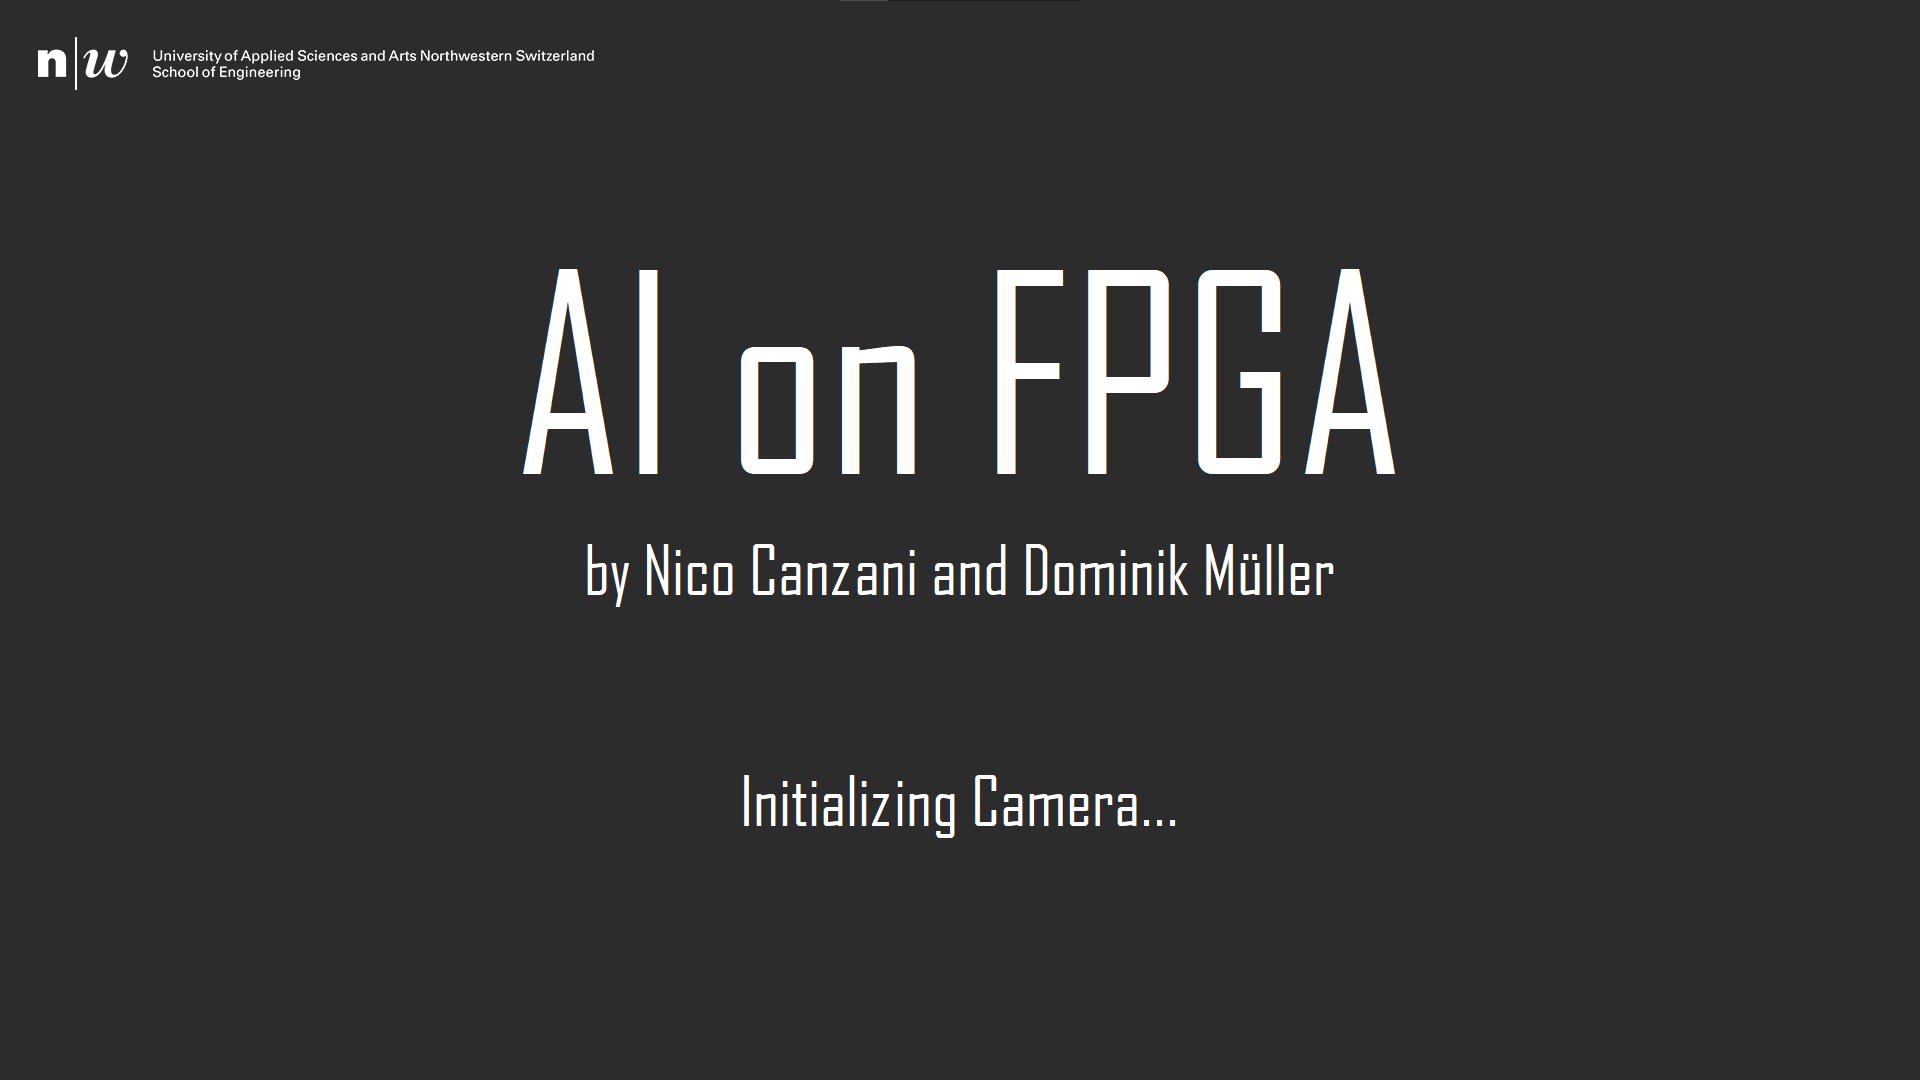
\includegraphics[width=\textwidth]{ui/ui_boot}
  \caption{Bootsplash screen with a camera initialization message}
  \label{fig:ui_boot}
\end{figure}

% \subsection{Inference Window}
% \label{subsec:inference:user_interface:inference_window}
\subsection{Inference Screen}
\label{subsec:inference:user_interface:inference_screen}

% The inference screen is shown after a throw has been detected and 
% The inference screen is shown after a detected throw has been inferred.
% The inference screen is shown after a detected throw has been evaluated.
The inference screen is displayed after a detected throw has been evaluated.
% For this purpose, the inference window consists of only three parts: the FHNW logo in the top left corner, an image of the throw and the classification statistics.
% For this purpose, the inference window consists of only three parts: the FHNW logo, an image of the throw and the classification statistics.
% For this purpose, the inference screen consists of only three parts: the FHNW logo, an image of the throw and the classification statistics.
% It consists of only three parts: the FHNW logo, an image of the throw and the classification statistics.
% It consists of the FHNW logo in the top left corner, an image of the throw on the left side and the classification statistics on the right side.
% It consists of the FHNW logo in the top left corner, an image of the throw on the left half of the screen and the classification statistics on the right half of the screen.
It consists of the FHNW logo in the top left corner, an acquired image of the object on the left half of the screen and the classification statistics on the right half of the screen.

% For this purpose, the frame with the highest, weighted prediction of the best guess is shown (see section \ref{subsec:inference:app:ui}).
% The displayed image of the object is the one with the highest weighted prediction of the best guess (see section \ref{subsec:inference:app:ui}).
% The displayed image of the object is the one with the highest weighted prediction of the class selected as the best prediction (see section \ref{subsec:inference:app:ui}).
The displayed image of the object is the one with the highest weighted prediction percentage of the class selected as the best prediction.
% This is usually an image of 
% usually a frame from the middle of the throw due to the weighting
% This is most likely a frame of the middle of the throw due to the weighting.
This is most likely a frame from the middle of the throw due to the applied weighting (see section \ref{subsec:inference:app:ui}).

% shows the best guess and up to 3 additional guesses as well as the rest of the classes summed up to 'Others'
% The classification statistics are visualized in a donut chart which shows the best guess, up to three additional guesses and the sum of the rest of the percentages.
The classification statistics are visualized in a donut chart which shows the best prediction, up to three additional predictions and the sum of the rest of the prediction percentages.
% A maximum of three additional guesses are shown, if there percentages are greater or equal to \SI{1.0}{\percent}.
% Additional guesses are only shown if there percentages are greater or equal to \SI{1.0}{\percent}.
Additional predictions are only shown if their percentages are greater or equal to \SI{1.0}{\percent}.
% The sum of the rest of the percentages is only shown if it is greater than zero after rounding.
% The sum of the rest of the percentages is only shown if it is not equal to zero after rounding.
Furthermore, the sum of the rest of the percentages is only shown if it is not equal to zero after rounding.
% All percentages are rounded to one decimal place when displayed (see section \ref{subsec:inference:app:ui}).
All percentages are rounded to one decimal place before being displayed (see section \ref{subsec:inference:app:ui}).

% Showing the required time for the image processing or the throughput is not really necessary as this time/speed in fps stays mostly constant
% (only background tasks can decrease the throughput)
% Displaying the required image processing time in milliseconds or the throughput in frames per second is not necessary.
Displaying the throughput of the image classification chain in frames per second is not necessary as it remains more or less constant.
% The small differences are a result of background tasks of the operating system.
The small differences are due to background tasks of the Linux operating system (see section \ref{sec:verification_and_benchmark:throughput}).

% Figure \ref{fig:ui_inference_paper_ball} show an example of the inference screen.
% Figure \ref{fig:ui_inference_paper_ball} show an example of the inference window.
Figure \ref{fig:ui_inference_paper_ball} show an example of the inference screen.
% However, the classifiaction accuracy is in most cases \SI{100.0}{\percent} and therefore the inference window usually looks like the one shown in figure \ref{fig:ui_inference_bunny}.
% The classifiaction accuracy, however, is \SI{100.0}{\percent} in most cases.
The classifiaction accuracy, however, reaches \SI{100.0}{\percent} in most cases.
% Therefore, the inference window usually looks like the one shown in figure \ref{fig:ui_inference_bunny}.
Therefore, the inference screen usually looks more like the one shown in figure \ref{fig:ui_inference_bunny}.
% this example and therefore the 

\begin{figure}
  \centering
  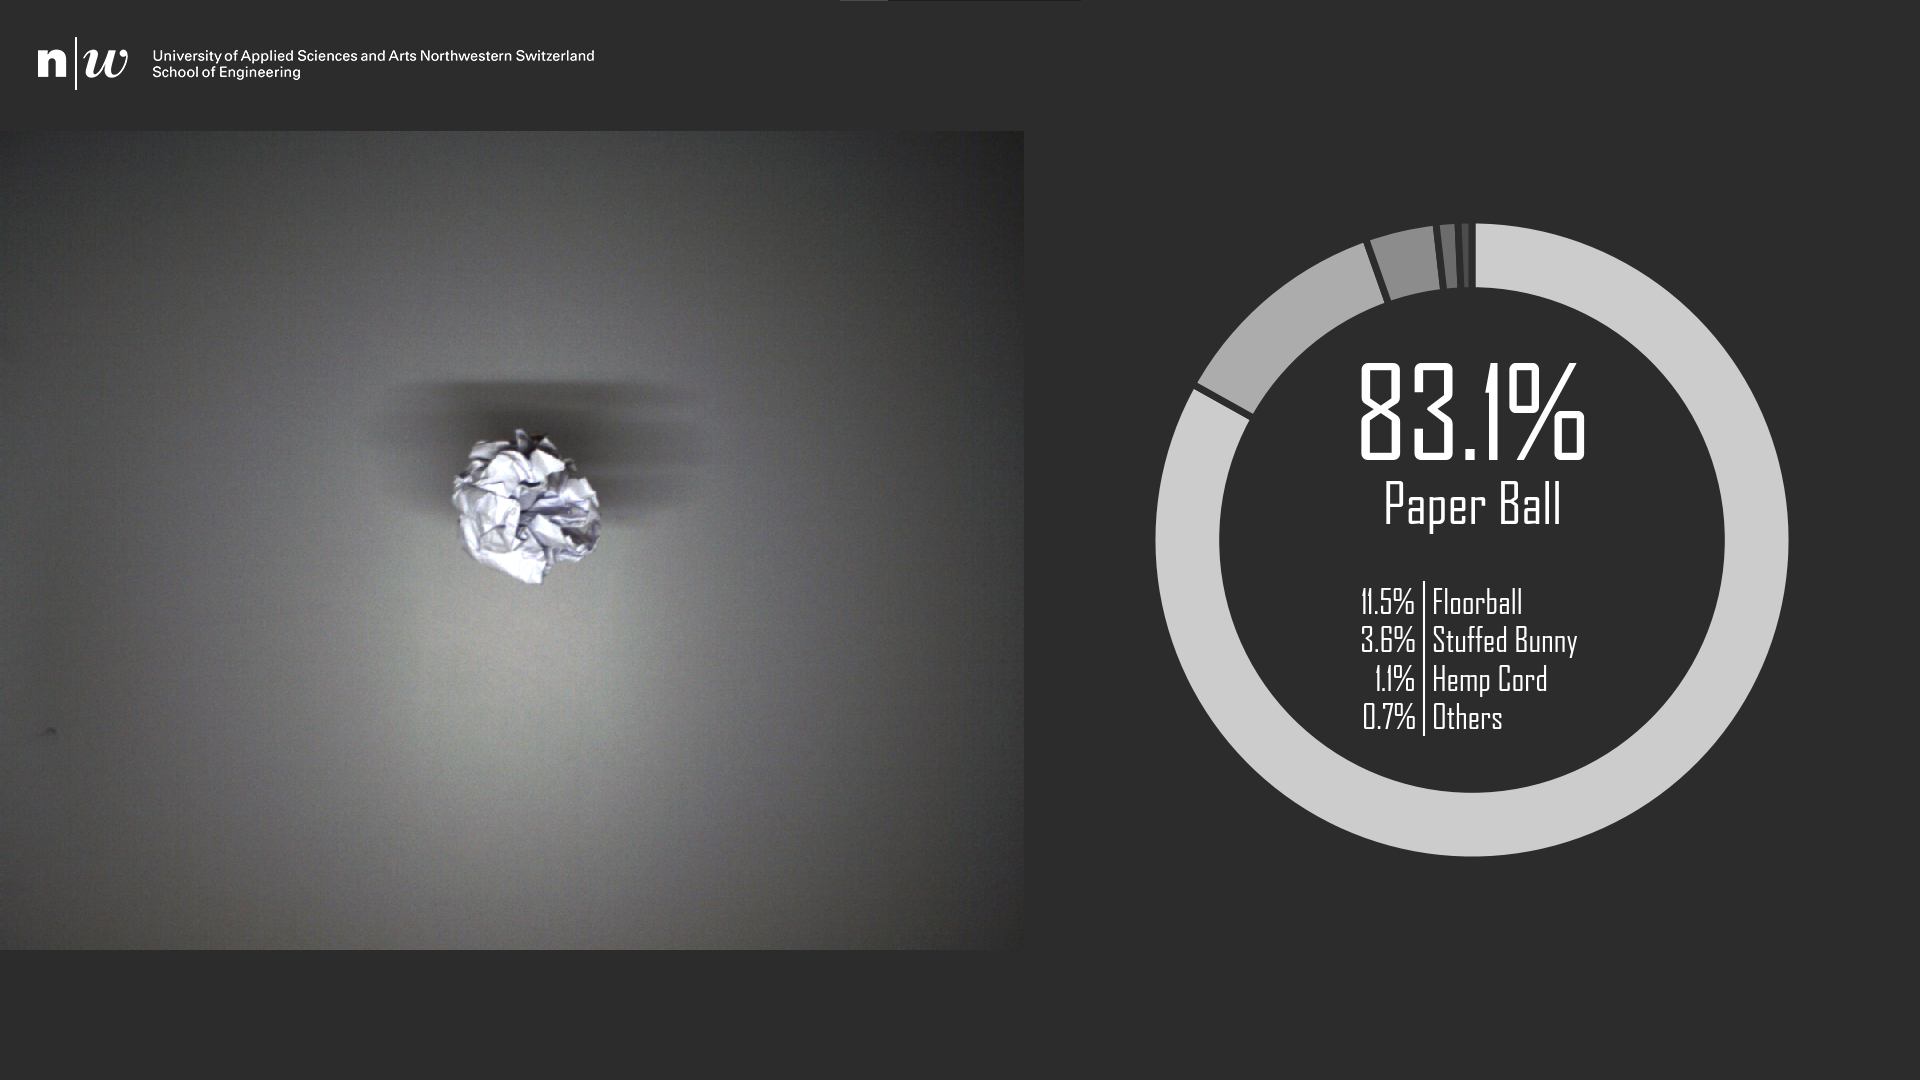
\includegraphics[width=\textwidth]{ui/ui_inference_paper_ball}
  \caption{Example of an inference screen showing the \textit{Paper Ball}}
  \label{fig:ui_inference_paper_ball}
\end{figure}

\begin{figure}
  \centering
  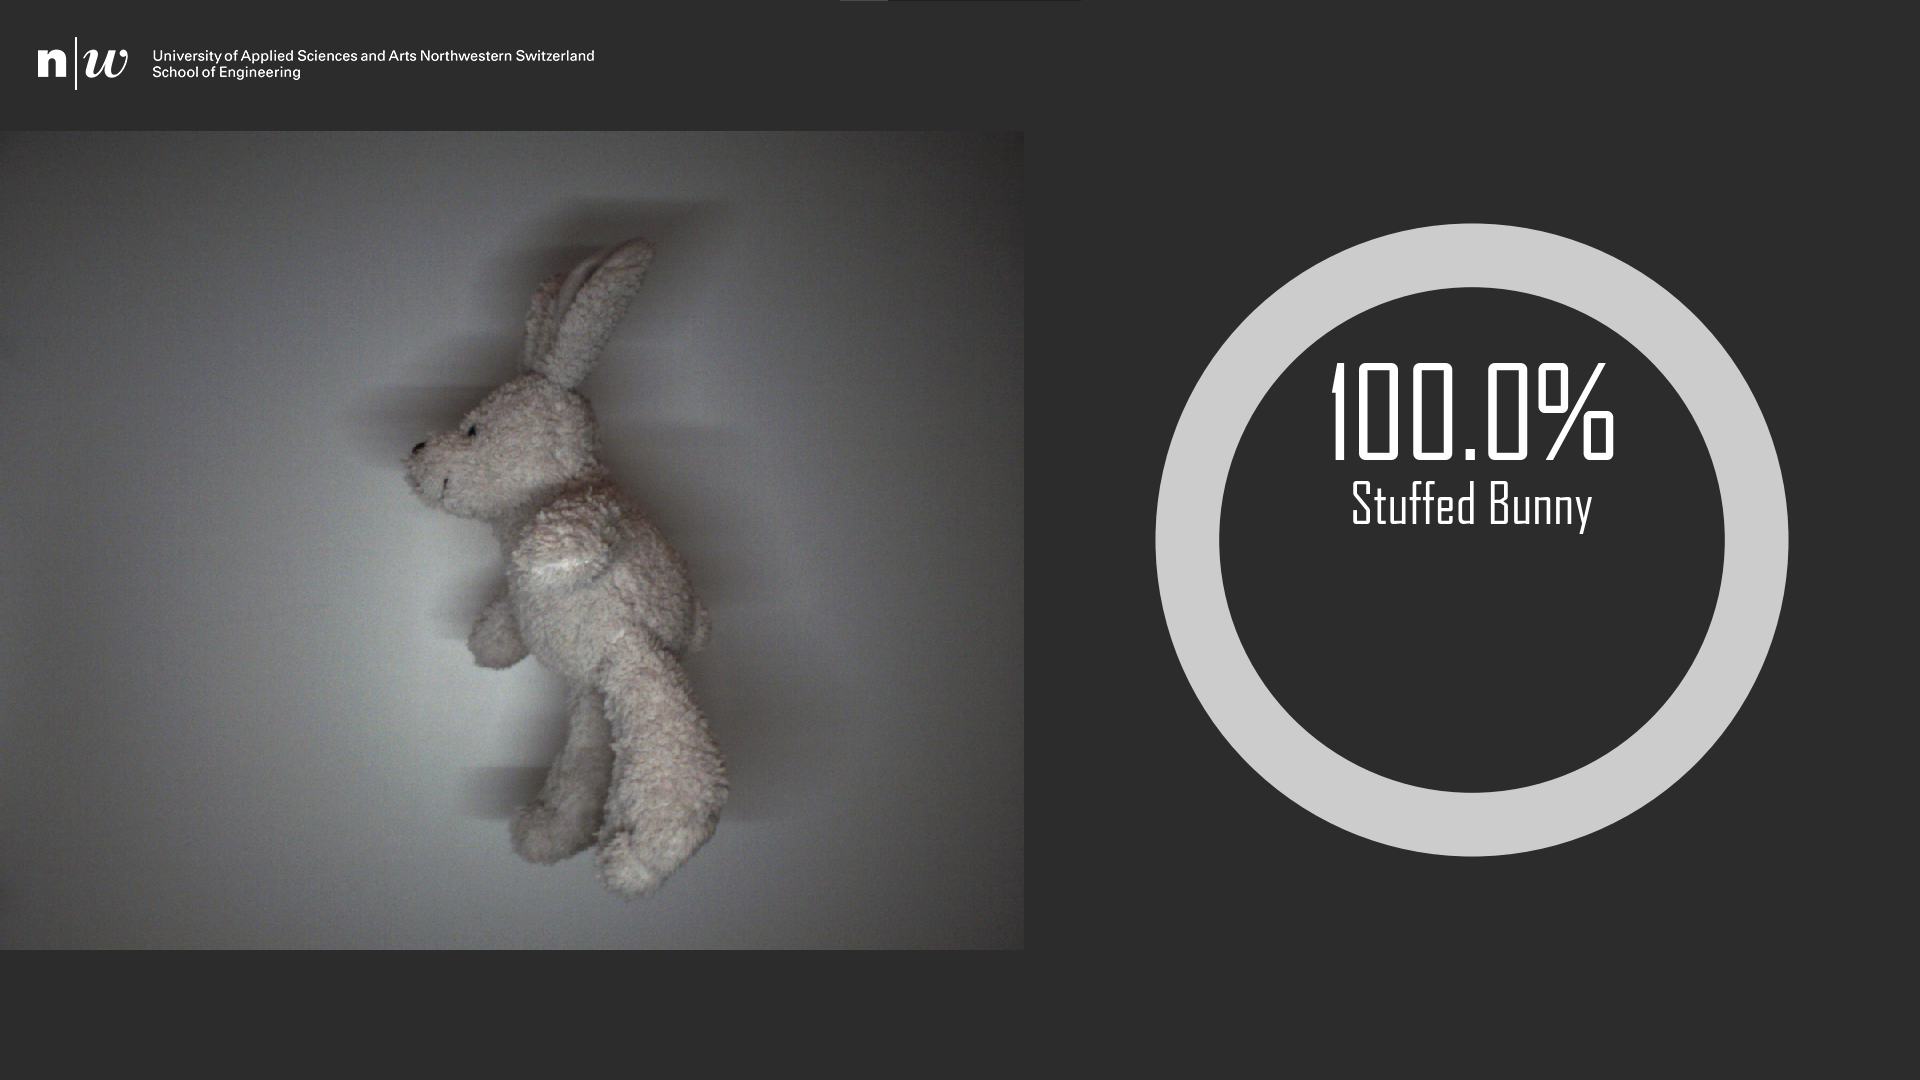
\includegraphics[width=\textwidth]{ui/ui_inference_bunny}
  \caption{Example of an inference screen with a prediction of \SI{100.0}{\percent}}
  \label{fig:ui_inference_bunny}
\end{figure}





\subsection{Implementation}
\label{subsec:inference:user_interface:implementation}

% implemented as a class with non-locking methos to update the screen
% done with PySimpleGUI
% Tkinter backend
% The user interface is implemented as a class in Python.
% The \acrlong{ui} is implemented as a class in the Python module \texttt{ui.py}.
% The implementation uses the Python packages PySimpleGUI and Matplotlib.
The \acrlong{ui} is implemented as a class in the Python module \texttt{ui.py} and uses the Python packages PySimpleGUI as well as Matplotlib.

PySimpleGUI allows for the creation of simple \acrlongpl{ui} that work across multiple platforms.
Currently, there exist four ports of PySimpleGUI and the Tkinter variant is used by default \cite{}. % todo: cite https://realpython.com/pysimplegui-python/
Tkinter is the standard Python interface to the Tk cross-platform widget toolkit that provides a library of graphical widgets to build \acrlongpl{ui} \cite{}. % todo: cite https://docs.python.org/3/library/tkinter.html

% with the help of the plotting library Matplotlib.
Matplotlib is a flexible plotting library which provides a MATLAB-like interface with the \texttt{pyplot} module.
% Even though it is easy to use, one is still able to tweak low-level 
% Even though it is easy to use, one still has full control over all the different properties of the plot \cite{}. % todo: cite https://matplotlib.org/3.1.1/index.html
Even though it is extremely easy to use, full control over the various properties is not sacrificed as low-level commands are also available \cite{}. % todo: cite https://matplotlib.org/3.1.1/index.html

% ------------------------------
\paragraph{User Interface Class}
The \texttt{UI} class consists of several non-blocking methods to update the \acrlong{ui} screens.
% Usually, PySimpleGUI would block the Python interpreter until a certain event is caused by user input.
% Usually, PySimpleGUI would block the Python interpreter until a user event occurs.
% The PySimpleGUI \texttt{Window} method \texttt{read} blocks the Python interpreter until a user event occurs (e.g. a button click).
% The PySimpleGUI \texttt{read} method of the \texttt{Window} class used to update the screens blocks the Python interpreter until a user event occurs (e.g. a button click).
Calling the PySimpleGUI \texttt{read} method of the \texttt{Window} class is used to update the screens.
However, this call blocks the Python interpreter until a user event occurs (e.g. a button click).
% This standard behaviour of \acrlongpl{ui} would make the entire package unusable.
This standard \acrlong{ui} behaviour would render the entire package unusable.
% Fortunately, the \texttt{read} method allows to specify a timeout, essentially turing it into polling mode.
% Fortunately, the \texttt{read} method allows to specify a timeout, which effectively puts it into polling mode.
Fortunately, the \texttt{read} method allows to specify a timeout, which essentially turns it into polling mode.
% Therefore, the \texttt{read} method is called with a short timeout of \SI{100}{ms} (necessary to update the screen) to create non-blocking methods.
% Therefore, the \texttt{read} method is called with a short timeout of \SI{100}{ms}, which is necessary to update the screen.
It is therefore called with a short timeout of \SI{100}{ms}, which is necessary to update the screen \cite{}. % todo: cite https://pysimplegui.readthedocs.io/en/latest/call%20reference/

The \texttt{boot\_window} and \texttt{inference\_window} methods are used to spawn windows with the appropriate layouts described in section \ref{subsec:inference:user_interface:bootsplash_screen} and \ref{subsec:inference:user_interface:inference_screen}.

The main methods are \texttt{update\_boot\_window} and \texttt{update\_inference\_window}.
% When called, they first check if the layout of the screen is set to the requested one and switch to it if necessary.
When called, they first check whether the screen layout is set to the requested one and switch to it if necessary.
% The \acrlong{ui} screen is then updated in a second step.
The \acrlong{ui} screen is then updated in a second step and requires the status message in case of the bootsplash screen.
% Updating the bootsplash screen only requires the status message (\texttt{message}) as a formal parameter.
% Updating the inference screen requires a list of the predictions, a list of the prediction percentages and the bytes encoded \acrshort{png} image
Updating the inference screen requires a list of the predictions, a list of the prediction percentages and the \acrshort{png} encoded image data.

% -----------------------------------
\paragraph{Classification Statistics}
% matplotlib.pyplot
% donut chart: (pie chart with circle of background color in the middle) / Pie Chart with an area of the centre cut out
% The classification statistics are displayed in the form of a donut chart.
% The \texttt{figure} method is used to create the donut chart.
% The \texttt{figure} method is used to turn the classification statistics into a donut chart.
The \texttt{figure} method uses Matplotlib to turn the classification statistics into a donut chart.
Directly generating a donut chart is, however, not possible with Matplotlib.
% However, directly generating a donut chart is not possible with Matplotlib.
% A pie chart with an area of the center cut out is therefore used.
% Therefore, a pie chart with a circle of the same color as the background at the center is used.
% Therefore, a pie chart with a circle in the background color at the center is used.
Therefore, a circle with the same color as the background is placed in the middle of a pie chart.
This simple modification creates the desired donut chart.

% To display the figure on the screen it has to be in the \acrshort{png} file format.
% To display a figure on the screen, it has to be in the \acrshort{png} file format.
% To display a figure on the screen, it must be in the \acrshort{png} file format.
To display the figure on the screen, it must be in the \acrshort{png} file format.
% For this reason, it is saved to a \texttt{bytes} buffer to avoid slow file operations.
For this reason, it is saved to an in-memory \texttt{bytes} buffer to avoid slow file operations.
This is implemented in the \texttt{get\_img\_from\_figure} method.

% no animation, processor is too slow, it would take too much time to render all the required frames to show an animation
% Animating the donut chart with Matplotlib would be very easy by rendering a few version of the donut chart overlayed with a circular sector in the background color.
% Animating the donut chart with Matplotlib would be very easy by rendering a few versions of the donut chart overlayed with a circular sector with the same color as the background.
% Animating the donut chart with Matplotlib would be very easy by rendering a few versions of the donut chart overlaid with circular sectors of the same color as the background.
% Animating the donut chart with Matplotlib would easily be possible by rendering a few versions of the donut chart overlaid with circular sectors of the same color as the background.
% Animating the donut chart with Matplotlib would easily be possible by rendering a few versions of it overlaid with circular sectors of the same color as the background.
% Animating the donut chart with Matplotlib would easily be possible by rendering several versions of it overlaid with circular sectors of the same color as the background.
% Animating the ring of the donut chart with Matplotlib would easily be possible by rendering several versions of it overlaid with a circular sector of the same color as the background.
Animating the ring of the donut chart with Matplotlib would easily be possible by rendering several versions of it overlaid with a circular sector in the background color.
% This would create the illusion that the ring is being drawn when played back.
% Starting at the top of the ring, the major sector can be decreased, starting at the top of the ring and progressing in a clockwise direction.
% The major sector can be decreased, starting at the top of the ring and progressing in a clockwise direction.
% The central angle can be decreased, starting at the top of the ring and progressing in a clockwise direction.
% As time progresses, the central angle is decreased, starting at the top of the ring and progressing in a clockwise direction.
% As time progresses, the central angle of the circular sector is decreased, starting at the top of the ring and progressing in a clockwise direction around the ring.
As time passes, the central angle of the circular sector is decreased, starting at the top of the ring and progressing in a clockwise direction around the ring.
% The ring can be overlayed with a circular sector, starting
% This would give the appearance that the ring is being drawn on the display when played back.
This would give the appearance that the ring is being drawn on the display.
% Unfortunately, the processor of the embedded system is not powerful enough to render several versions of the statistics in a reasonable amount of time.
Unfortunately, the processor of the embedded system is not powerful enough to render several versions of the donut chart in a reasonable amount of time.
% The processor of the embedded system is unfortunately not powerful enough to render several versions of the statistics in a reasonable amount of time.
% For this reason, the statistics cannot be animated.

% ----------------
\paragraph{Cursor}
% The cursor cannot be disabled globally, it is, however, possible to hide it when hovering over certain elements.
% The cursor cannot be disabled globally, but it is possible to hide it when hovering over certain elements.
The cursor cannot be disabled globally, but it is possible to hide it when is is hovering over certain elements (e.g. text, images).
% For this purpose, the underlying Tkinter widgets can be accessed with the \texttt{Widget} class variable.
For this purpose, the underlying Tkinter widgets are accessed with the \texttt{Widget} class variable and the cursor is set to invisible \cite{}. % todo: cite https://pysimplegui.readthedocs.io/en/latest/#widget-access
% ---- cursor stays at the same place
% The position of the cursor is centered on the screen after 
% After booting, the position of the cursor is centered on the screen and the respective Tkinter widgets are modified.
% After booting, the position of the cursor is centered on the screen.
The cursor position is centered on the screen after booting.
Therefore, the respective Tkinter widgets located in the center are modified to hide the cursor.
